
\documentclass{beamer}

\newcommand*{\mybox}[1]{\framebox{#1}}

\mode<presentation> {
\usetheme{CambridgeUS}
\usecolortheme{dolphin}
}

\usepackage{graphicx} 
\usepackage{booktabs} 

\title[Gerez, Riaz \& Teoldi]{The structure of inequality and politics of redistribution} 

\author{Lupu and Pontusson (2011)} 
\institute[] 
{
Julian Enrique Gerez, Zara Riaz \& Filippo Teoldi \\ \medskip

}
\date{October 23, 2018} 

\begin{document}
\begin{frame}
\titlepage 
\end{frame}
\begin{frame}
\frametitle{Outline} 
\tableofcontents 
\end{frame}

\begin{frame}
\frametitle{Countries}
Countries sample
\begin{center}
\includegraphics[scale=0.45]{countries}
\end{center}
\end{frame}

\begin{frame}

\subsection{Aim of the paper}
\frametitle{Aim of the paper}
\begin{itemize}
\item [1.]  Redistributive policy outcomes correspond to the policy preferences of middle-income voters, 
\medskip
\item[2.] The structure of the inequality helps explain why the preferences of middle-income voters vary across countries and over time,
\medskip
\medskip
\medskip
\begin{center}
$\rightsquigarrow$  Does the structure of  \textbf{inequality} lead to more \textbf{redistribution}? \\
\end{center}
\medskip
\end{itemize}
\end{frame}

\begin{frame}
\frametitle{Inequalities and Social affinity hypothesis}
\begin{itemize}
\item[•] Structure of inequality, rather than the level: 
\textbf{Skew} = $\frac{90th/50th}{50th/10th}$ 
\medskip

\begin{center}
\begin{frame}
\frametitle{DAG}
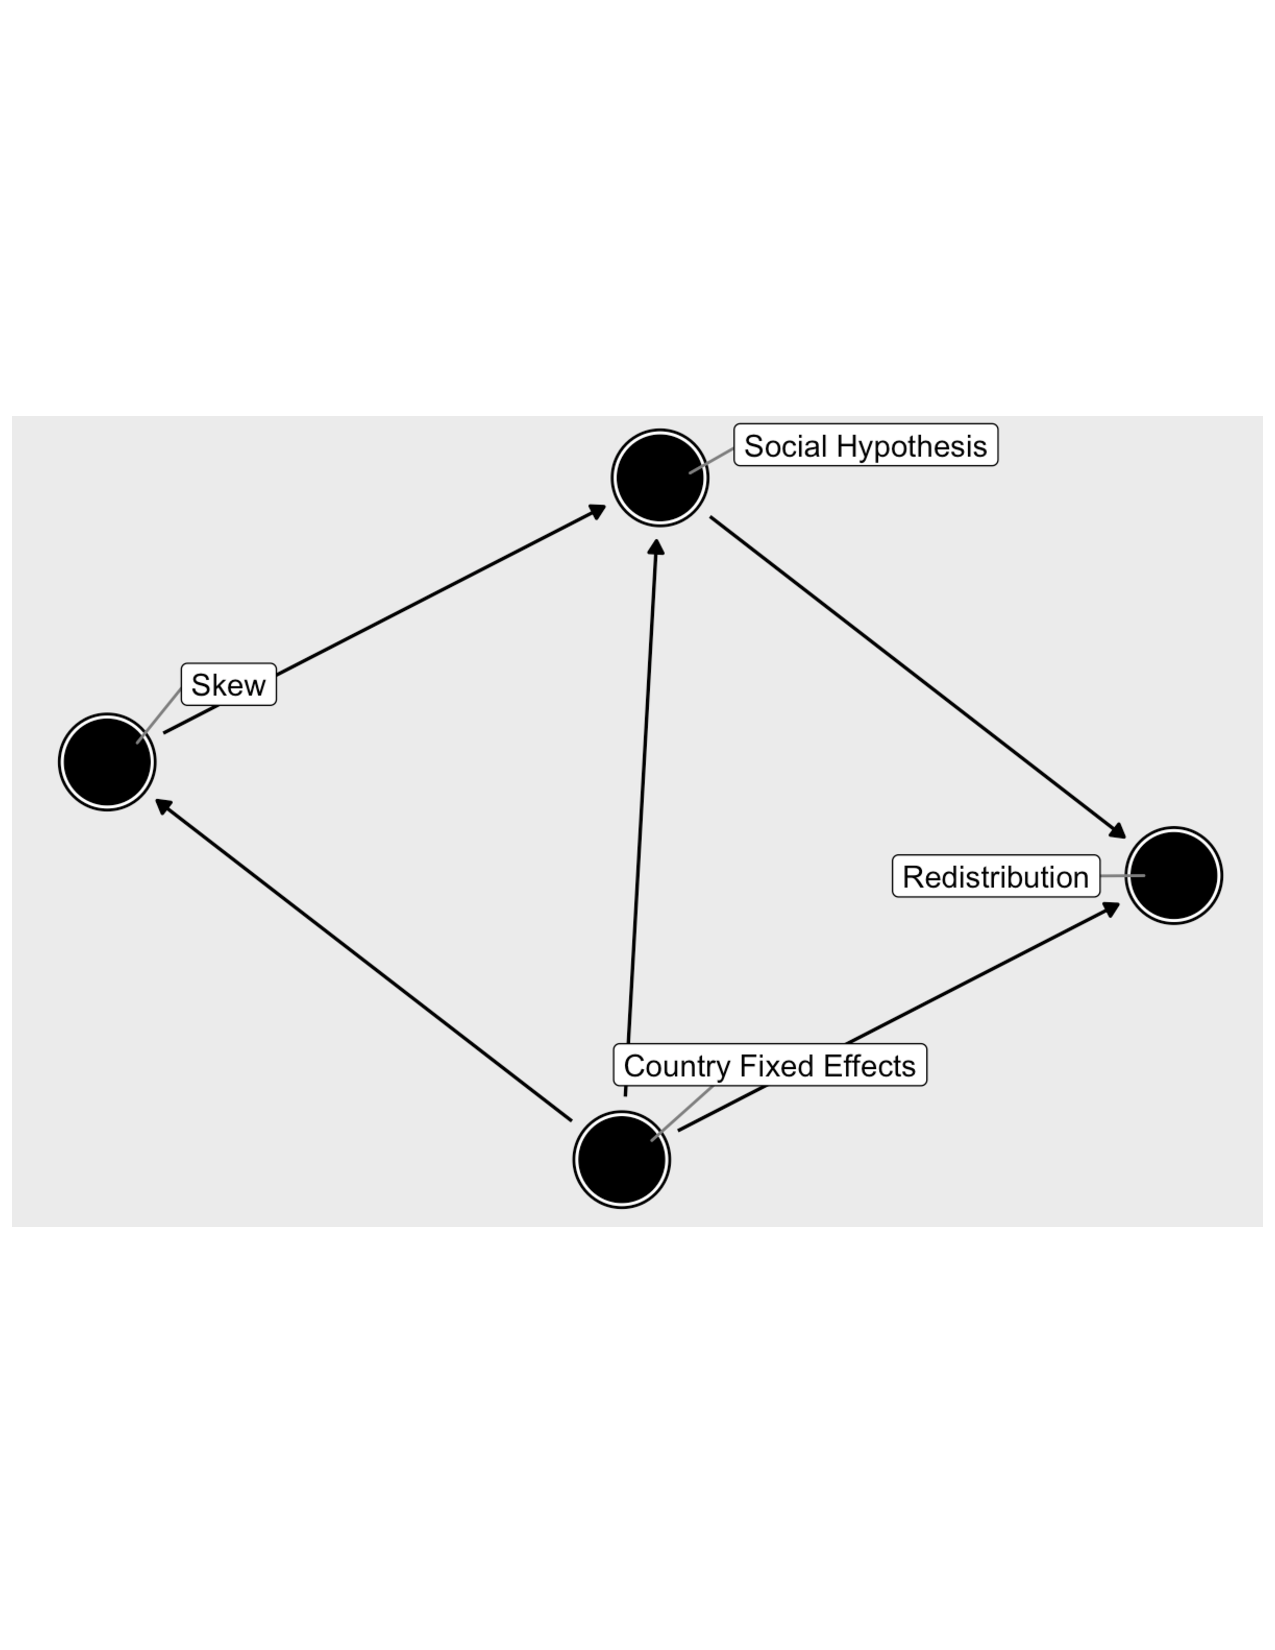
\includegraphics[scale=0.5]{dags}
\end{frame}
\end{center}
\begin{frame}
\subsection{Design declaration} 
\frametitle{Design Declaration}\
* Model (M): The paper tests the social affinity hypothesis that predicts middle-income voters will support redistribution policies when the distance between the middle and poor is small relative to the distance between the middle and the affluent (skew). (pg. 317)

* Inquiry (I): The study attempts to estimate parameter β from the simple model:

$$
y_i = \alpha + \beta x_i + \epsilon
$$

* This can be conceptualized as the summary of all potential outcomes across conditions $\beta$ for all units. More specifically, this would be all potential outcomes of redistribution conditional on inequality measured in a variety of ways, such as skew. We assume that this model describes the true data generating process.

* Data Strategy (D): The study uses country-year data on redistribution (% change in Gini coefficients brought about by taxes and government transfers) and non-elderly social spending for 18 OECD countries for the period 1969-2005. The data is purely observational and does not involve sampling. We focus on the measure of *skew* in particular.

* Answer Strategy (A): The authors use a variety of different answer strategies. Their model specifications can be constructed from variations on:

$$
R_{i,t} = \alpha + \beta X_{i,t} + \theta Y_{i,t} + \gamma R_{i, t-1} + \epsilon_{i,t}
$$

* Where for each country $i$ and year $t$, $R_{i,t}$ refers to redistribution, $\alpha$ is the constant, $\beta$ is the coefficient for skew, $X$, $\theta$ is the coefficient for the level of inequality, $Y$, $\gamma$ is the coefficient for redistribution lagged by one year ($R_{i,t-1}$) and $\epsilon_{i,t}$ is the error term. In different models the authors either use a vector of control variables or country fixed effects.

\end{frame}



\begin{frame}
\frametitle{Empirical results}
$\longrightarrow$ Redistribution
\begin{center}
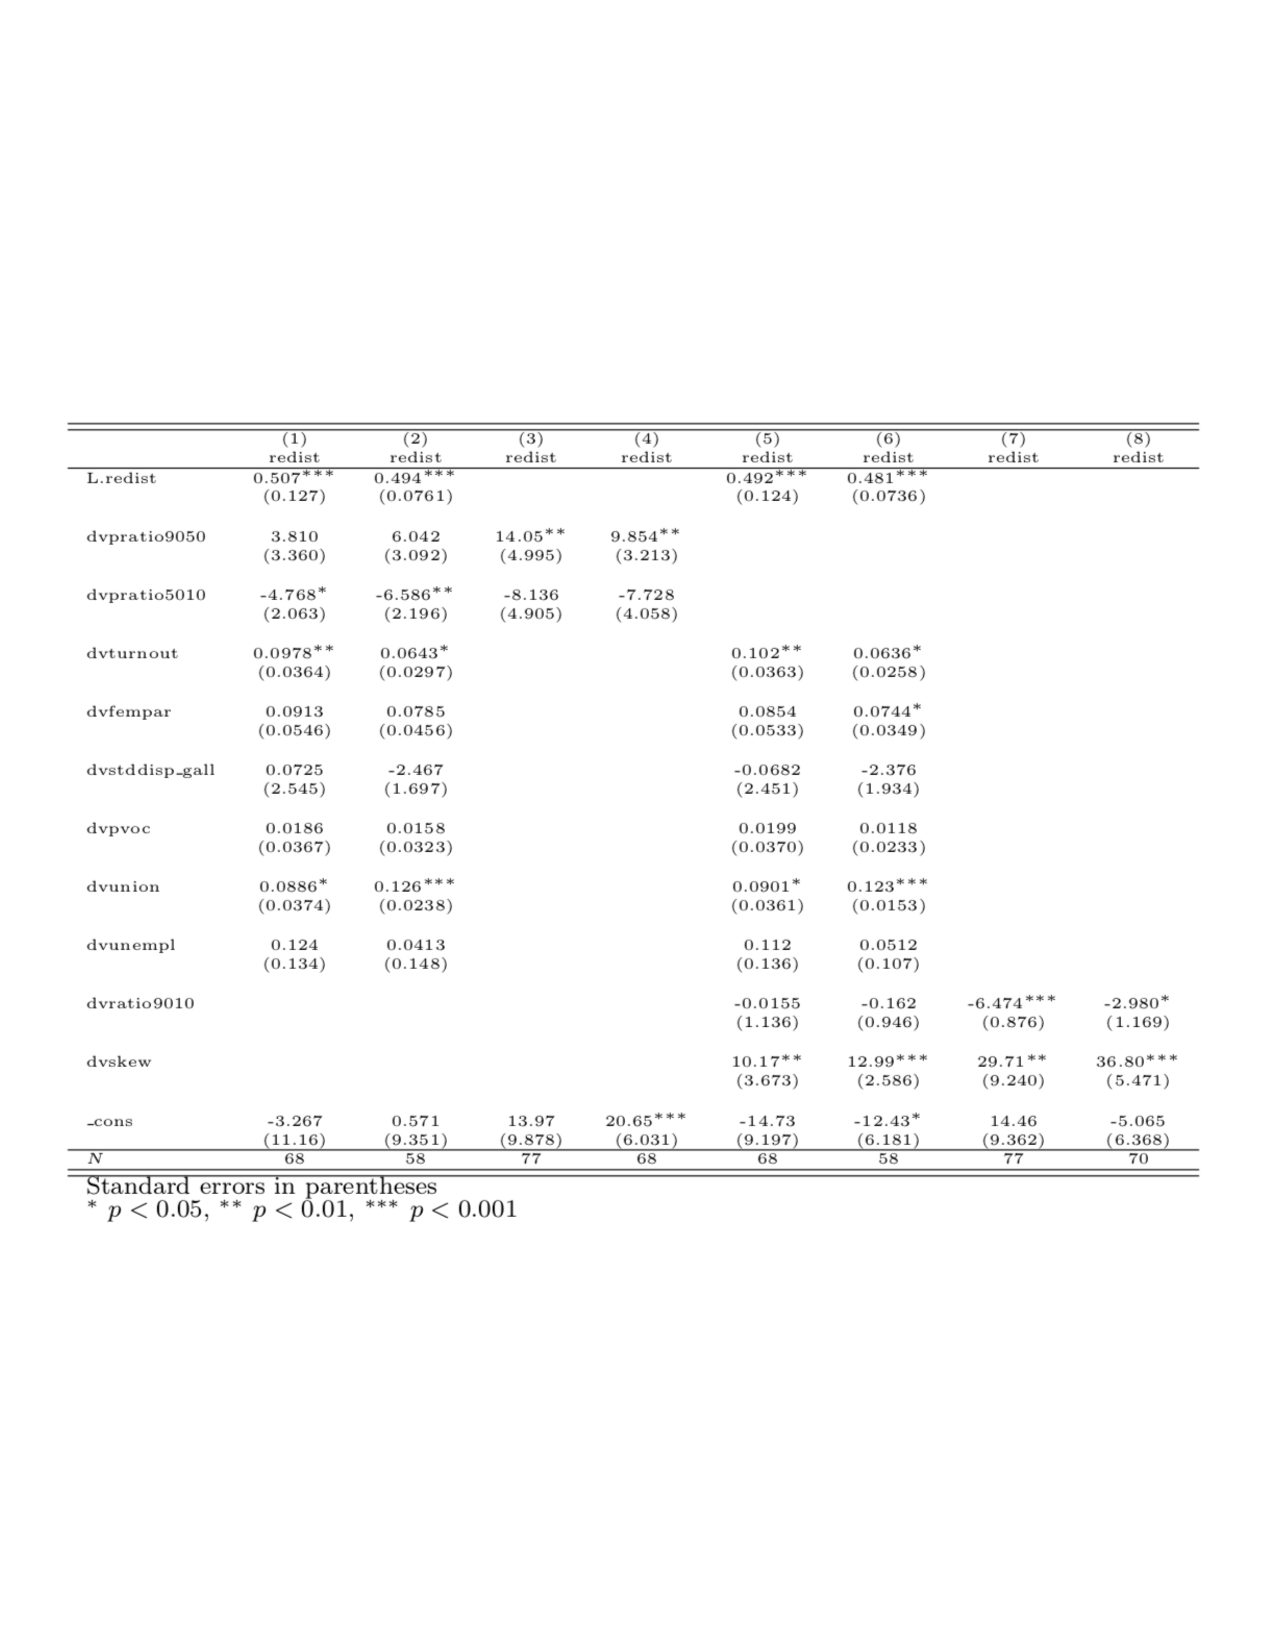
\includegraphics[scale=0.35]{tab2}
\end{center}
\end{frame}

\begin{frame}
\frametitle{Empirical results}
$\longrightarrow$ Social spending
\begin{center}
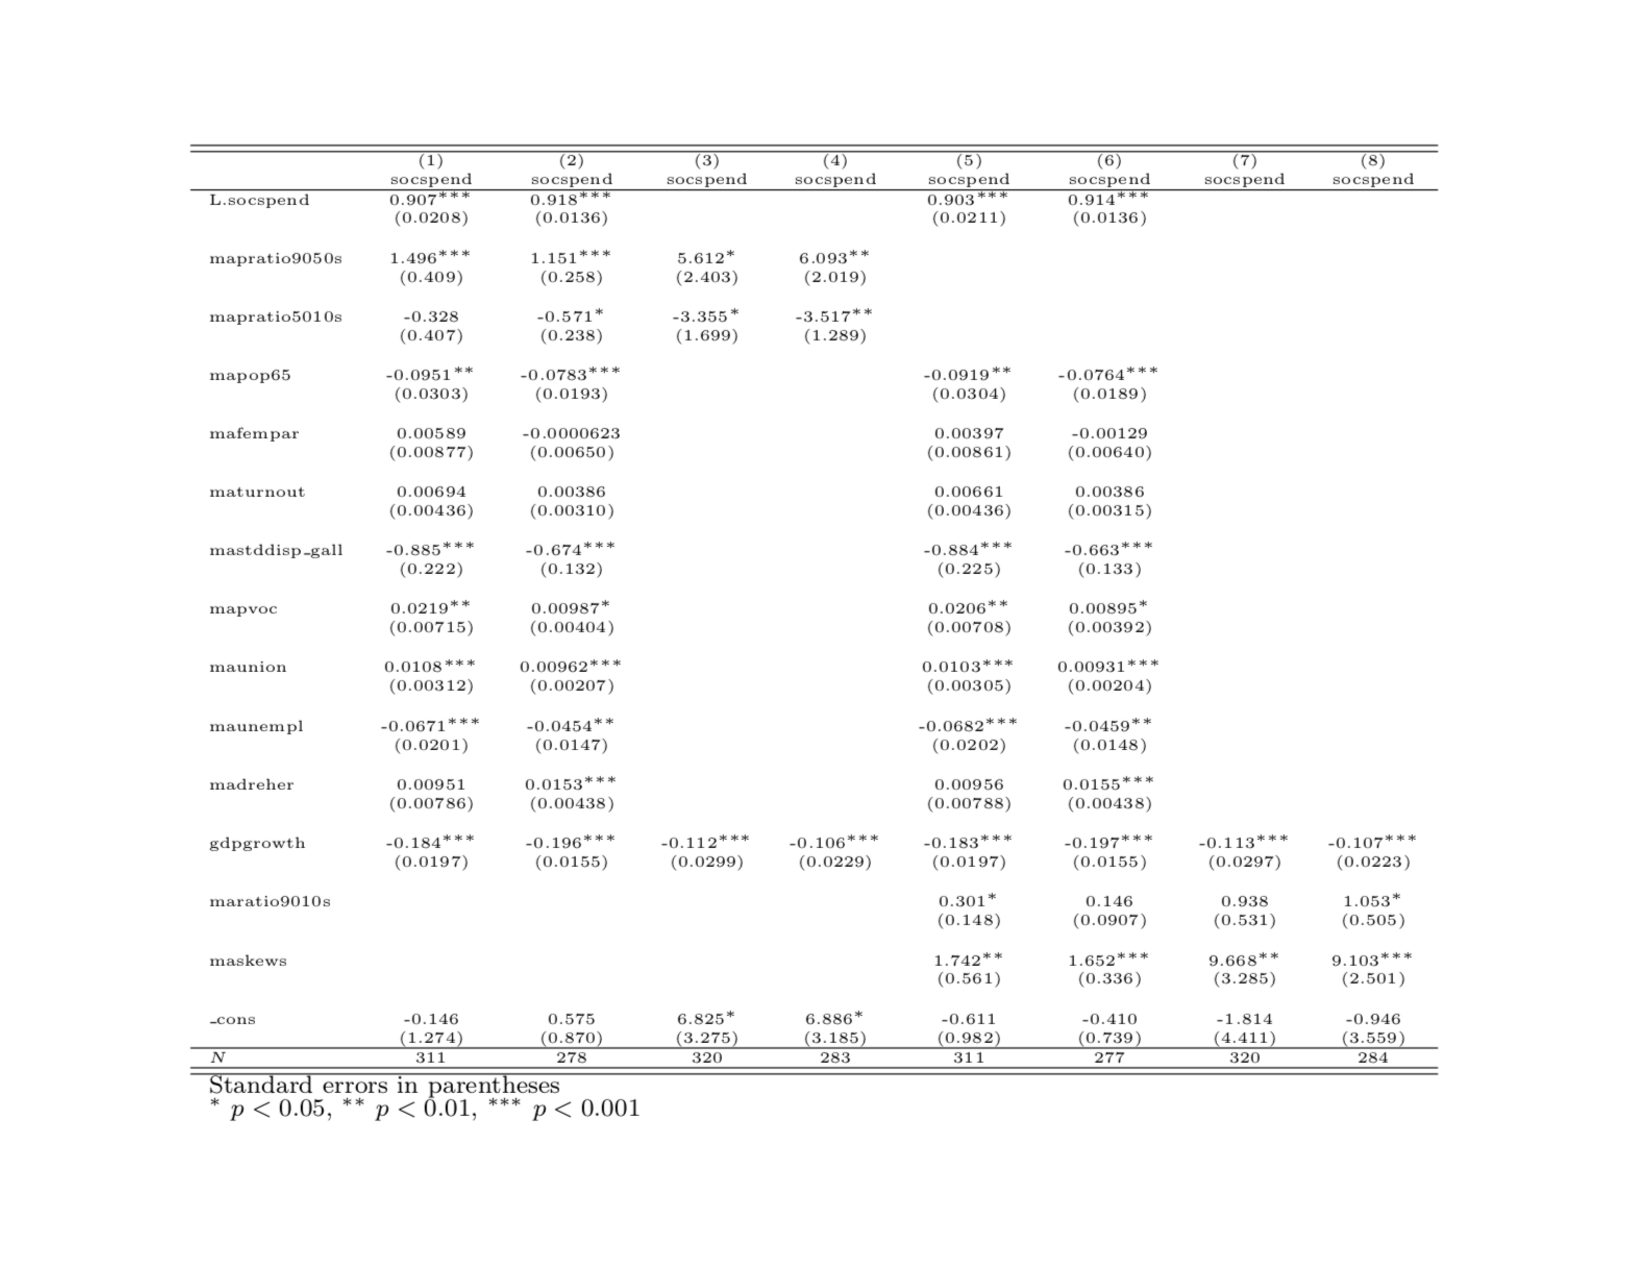
\includegraphics[scale=0.35]{tab3}
\end{center}
\end{frame}


\begin{frame}
$\longrightarrow$  Robust evidence that \textbf{structure of inequality} is significantly associated with redistribution\\
\medskip
\medskip
$\longrightarrow$ \textbf{redistribution increases} with dispersion of the upper half of the earnings distribution and with compression of the lower half of the earnings distribution
\end{frame}


\begin{frame}
\subsection{Robustness check} 
\frametitle{Robustness check}
As robustness checks, we re-estimate table 2 and 3 of the paper, using:
\begin{itemize}
\item[1] AR(1)-type autocorrelation structure correlation with a unique correlation coefficient for each panel (psar1)
\item[2] Different panel correction methods (a = Huber-White sandiwch estimator, b = panel-weighted least squares) 
\end{itemize} 
\medskip
$\longrightarrow$  consistent with the original paper's results 
\medskip
\medskip
\begin{itemize} 
\item[•] \textbf{Tabel 2 and 3 with a) autocorr, psar1 and b1) phet Huber White and b2) phet NP1}
\end{itemize}
\end{frame}


\begin{frame}
\subsection{Extensions} 
\frametitle{Extensions}\
\begin{itemize}
\item[•] We disaggregate OECD data for social spending. In particular, public spending on:
\medskip
\begin{itemize}
\item[-] Family benefits
	\begin{itemize}
	\item Child-related transfers
	\item Public spending on services for families with children
	\item Financial support for these families through the tax system
	\end{itemize}
\item[-] Incapacity spending
\begin{itemize}
	\item Spending due to sickness, disability, and occupational injury
	\item Spending on occupational injury and disease
	\item Spending on services such as day care, rehabilitation, and home-help services
	\end{itemize}
\item[-] Labor market  spending (i.e. training, hiring subsidies and direct job creations)
\begin{itemize}
	\item Public employment services (PES)
	\item Training and hiring subsidies
	\item Direct job creations in the public sector
	\item Spending on services such as day care, rehabilitation, and home-help services
	\end{itemize}
\item[-] Unemployment benefits
\end{itemize} 
\end{itemize}
\end{frame}


\begin{frame}
\frametitle{Family benefits}\
\begin{center}
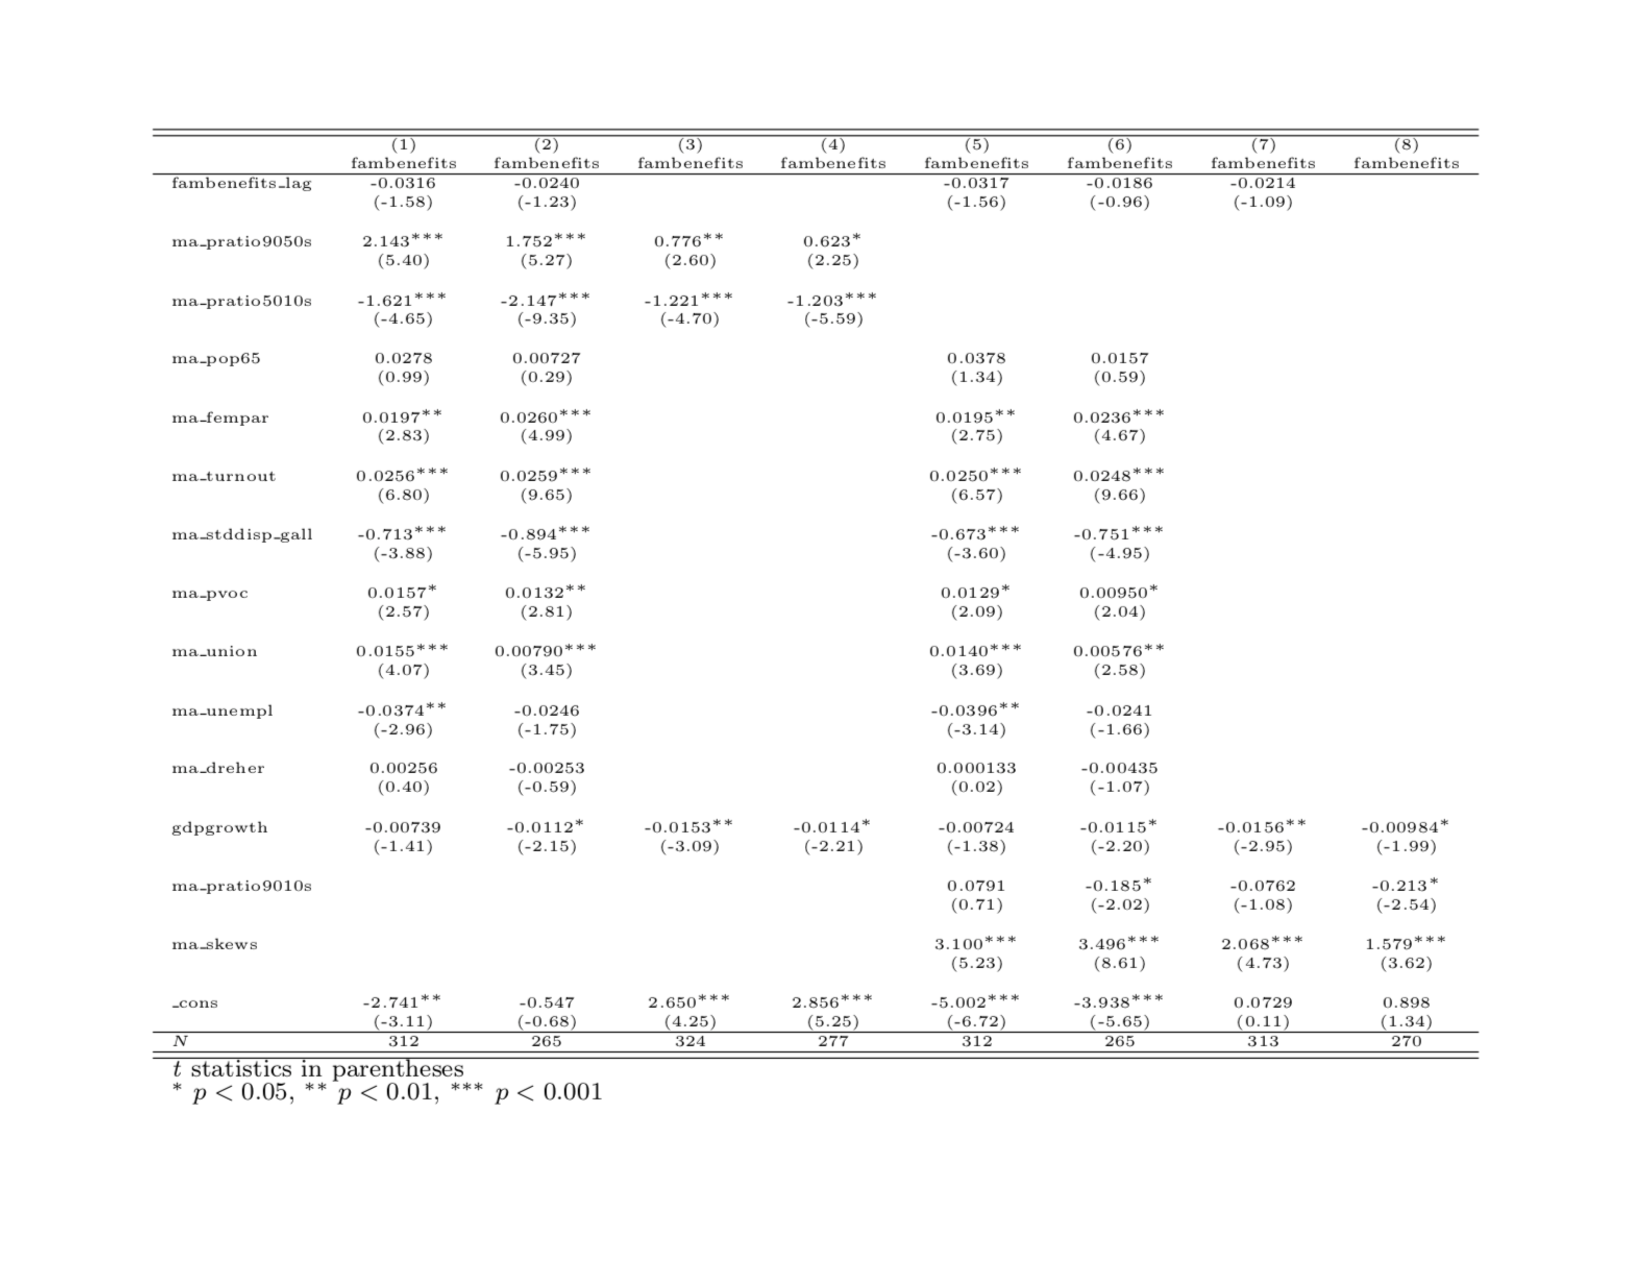
\includegraphics[scale=0.35]{family}
\end{center}
\end{frame}


\begin{frame}
\frametitle{Incapacity}\
\begin{center}
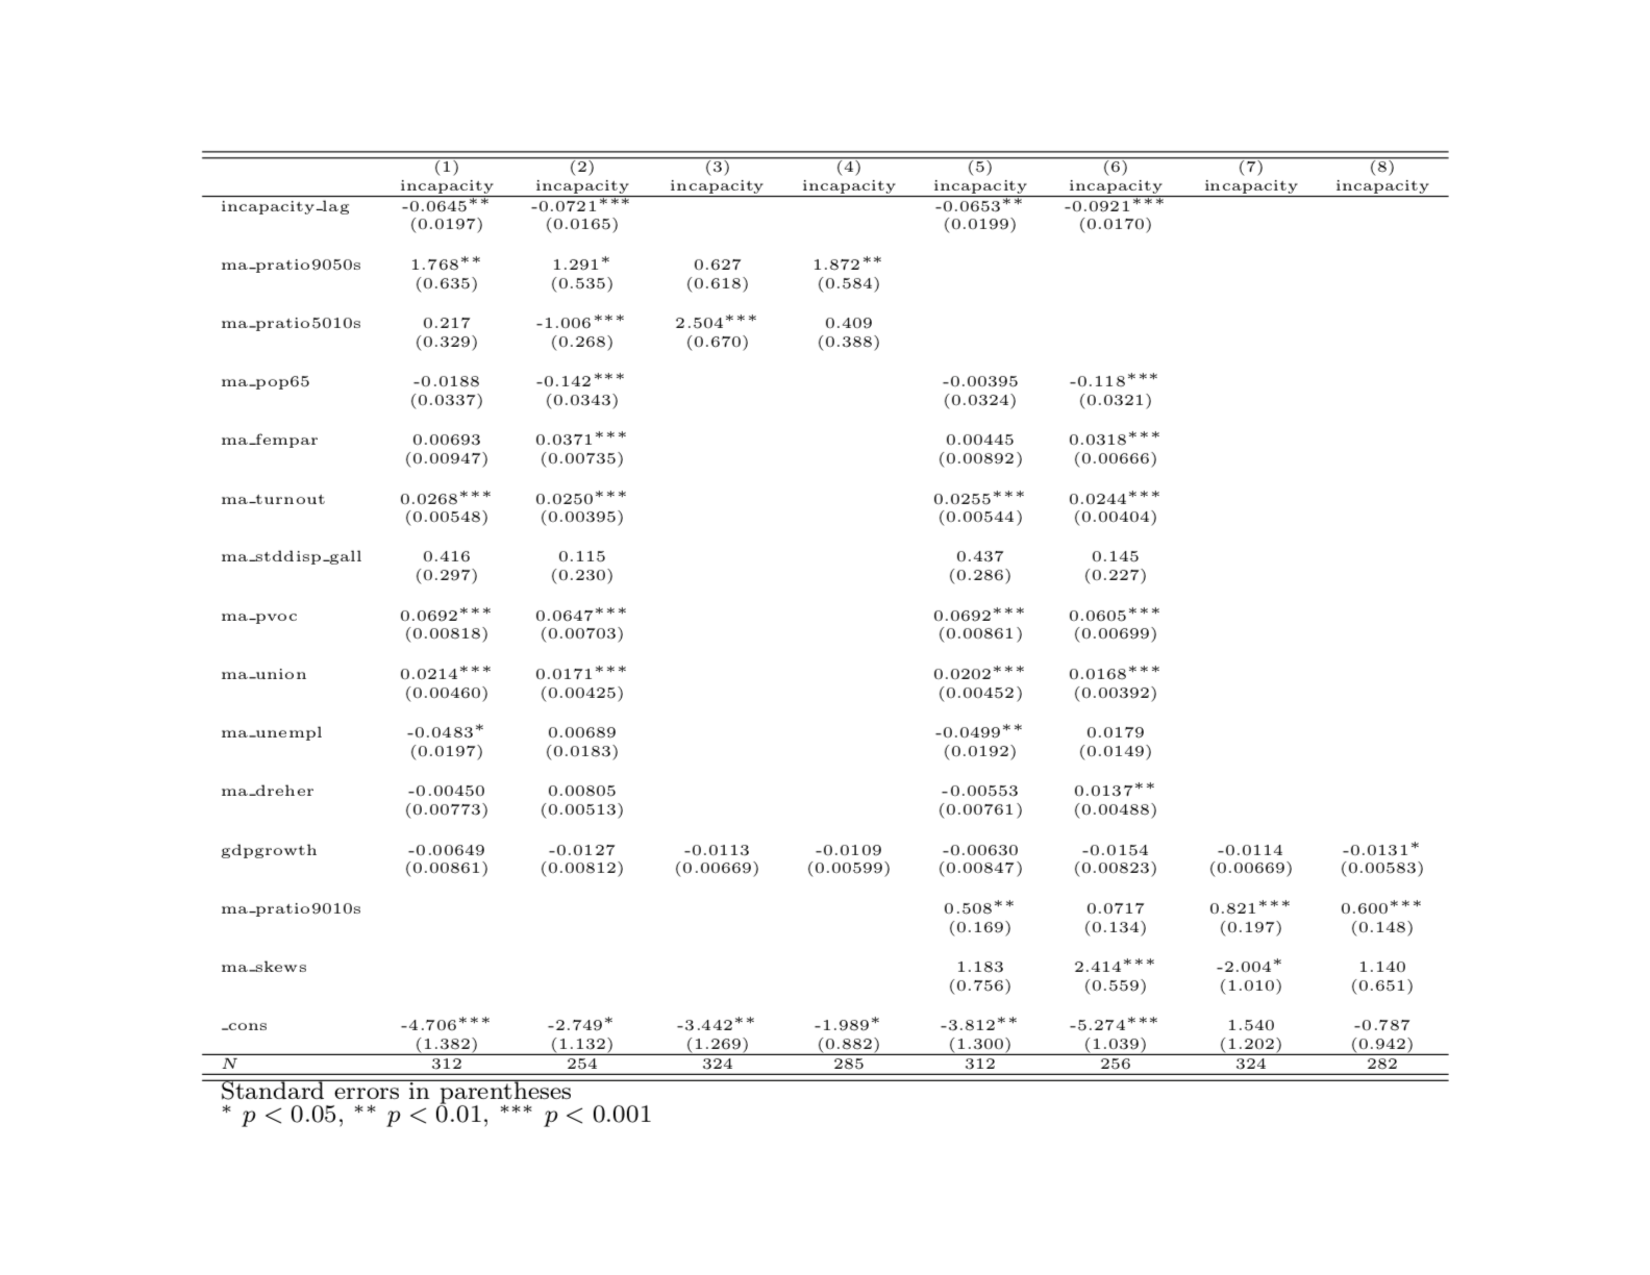
\includegraphics[scale=0.35]{incapacity}
\end{center}
\end{frame}

\begin{frame}
\frametitle{Public Spending on Labor}\
\begin{center}
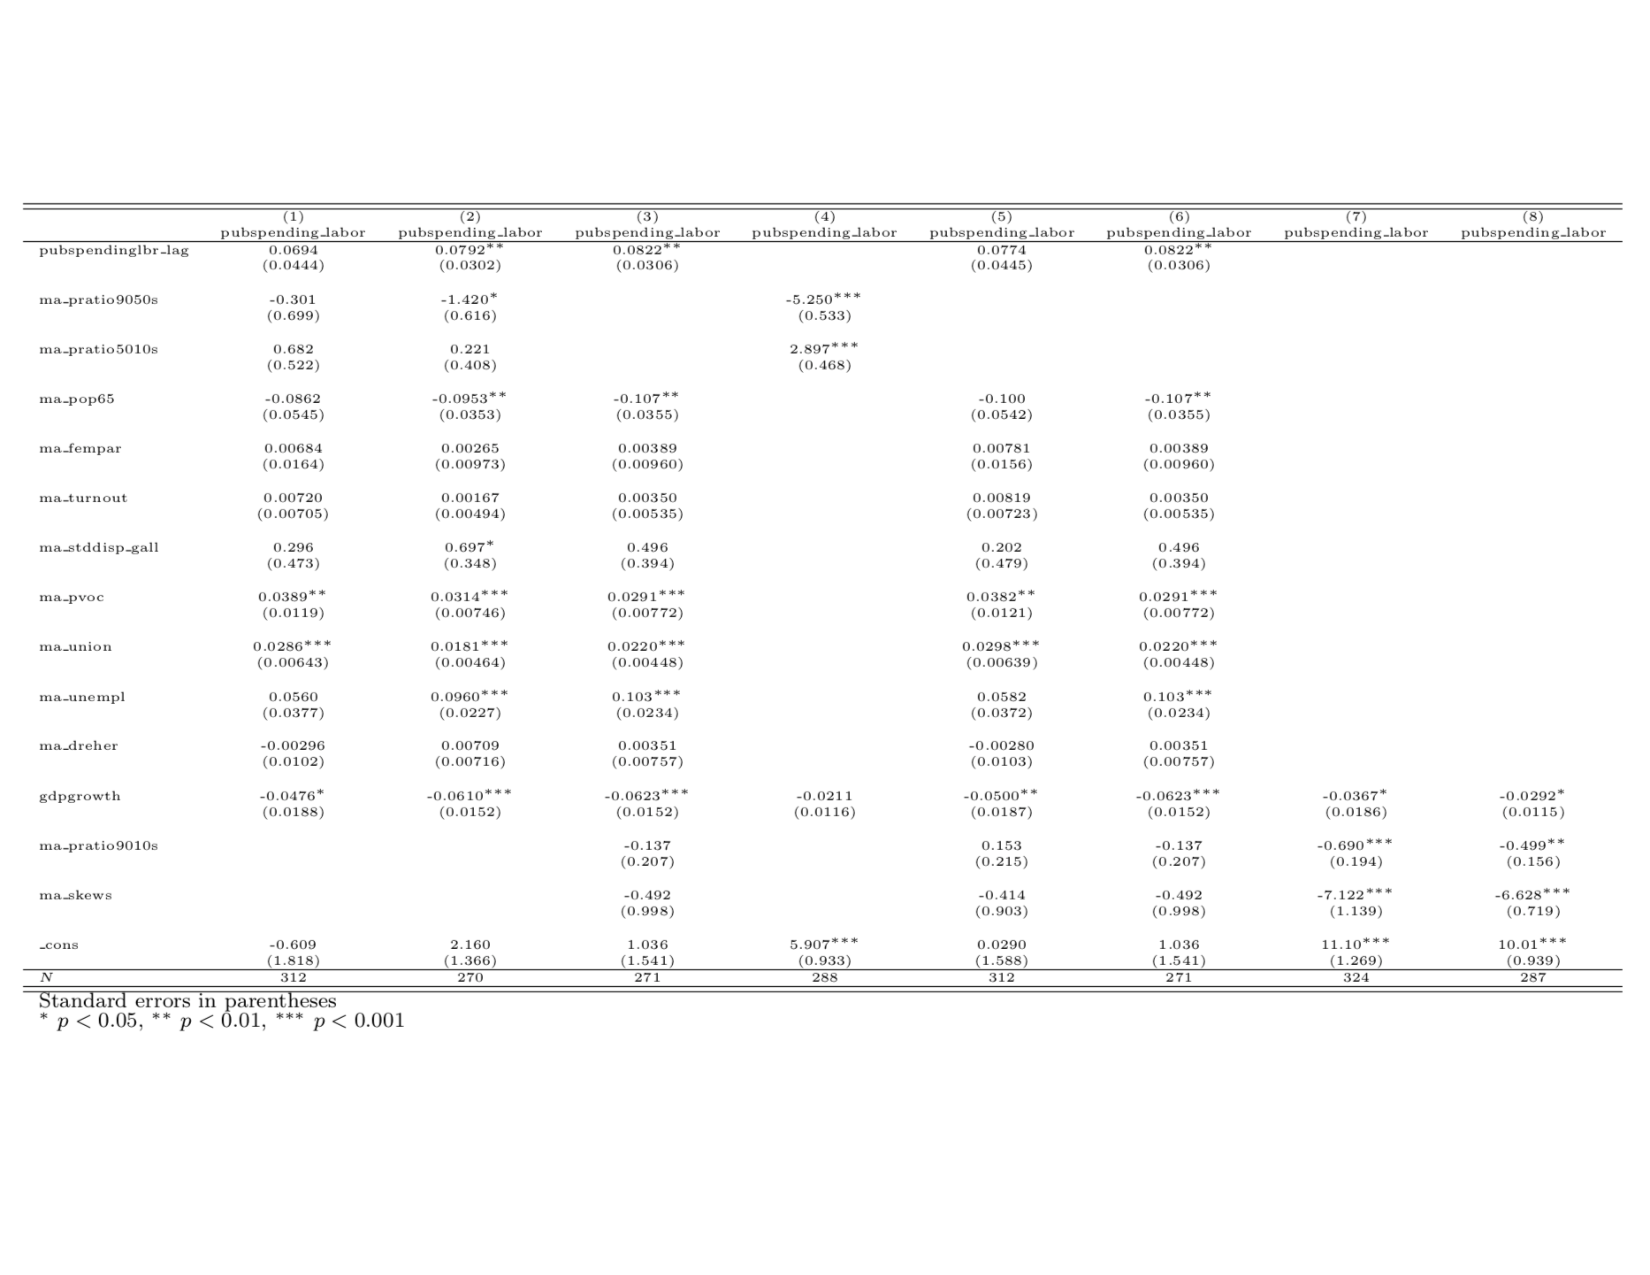
\includegraphics[scale=0.35]{exp}
\end{center}
\end{frame}

\begin{frame}
\frametitle{Unemployment benefits}\
\begin{center}
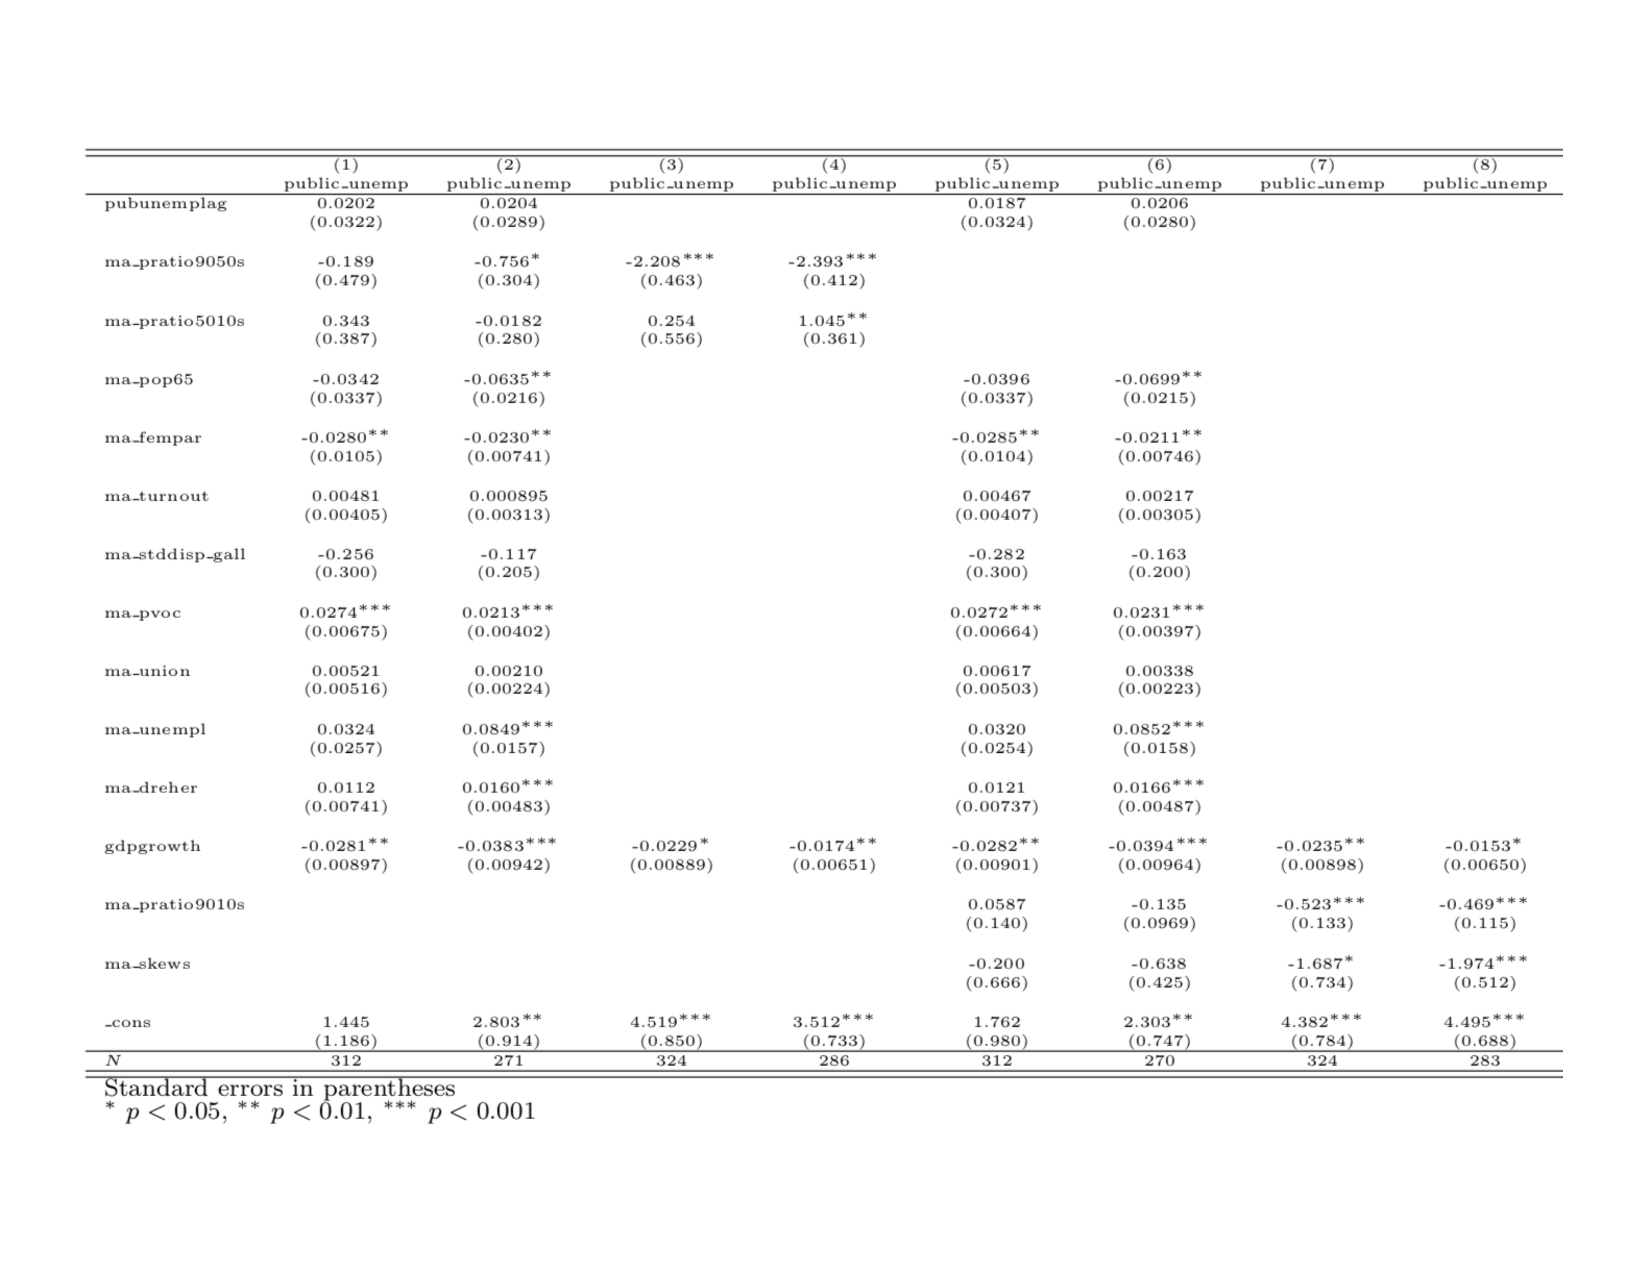
\includegraphics[scale=0.35]{bene}
\end{center}
\end{frame}


\begin{frame}
\subsection{Conclusion}
\frametitle{Conclusion}
\begin{itemize}
\item[1.] The structure of \textbf{inequality} is statistically and significantly associated with greater \textbf{redistribution and social spending}.
\medskip
\medskip
\medskip
\item[2.] \textbf{Middle-income voters} are incline to allay with low-income voters and support redistributive policies when the distance between the middle and the poor is small (relative to the distance between the middle and the upper).
\medskip
\medskip
\medskip
\item[3.] \textbf{Left-leaning governments} are more likely to redistribute income than right-leaning government s and  governments are more likely to be left-leaning when the structure of inequality is skewed.
\end{itemize}
\end{frame}

\begin{frame}
\frametitle{Disaggregation Results}
\begin{center}
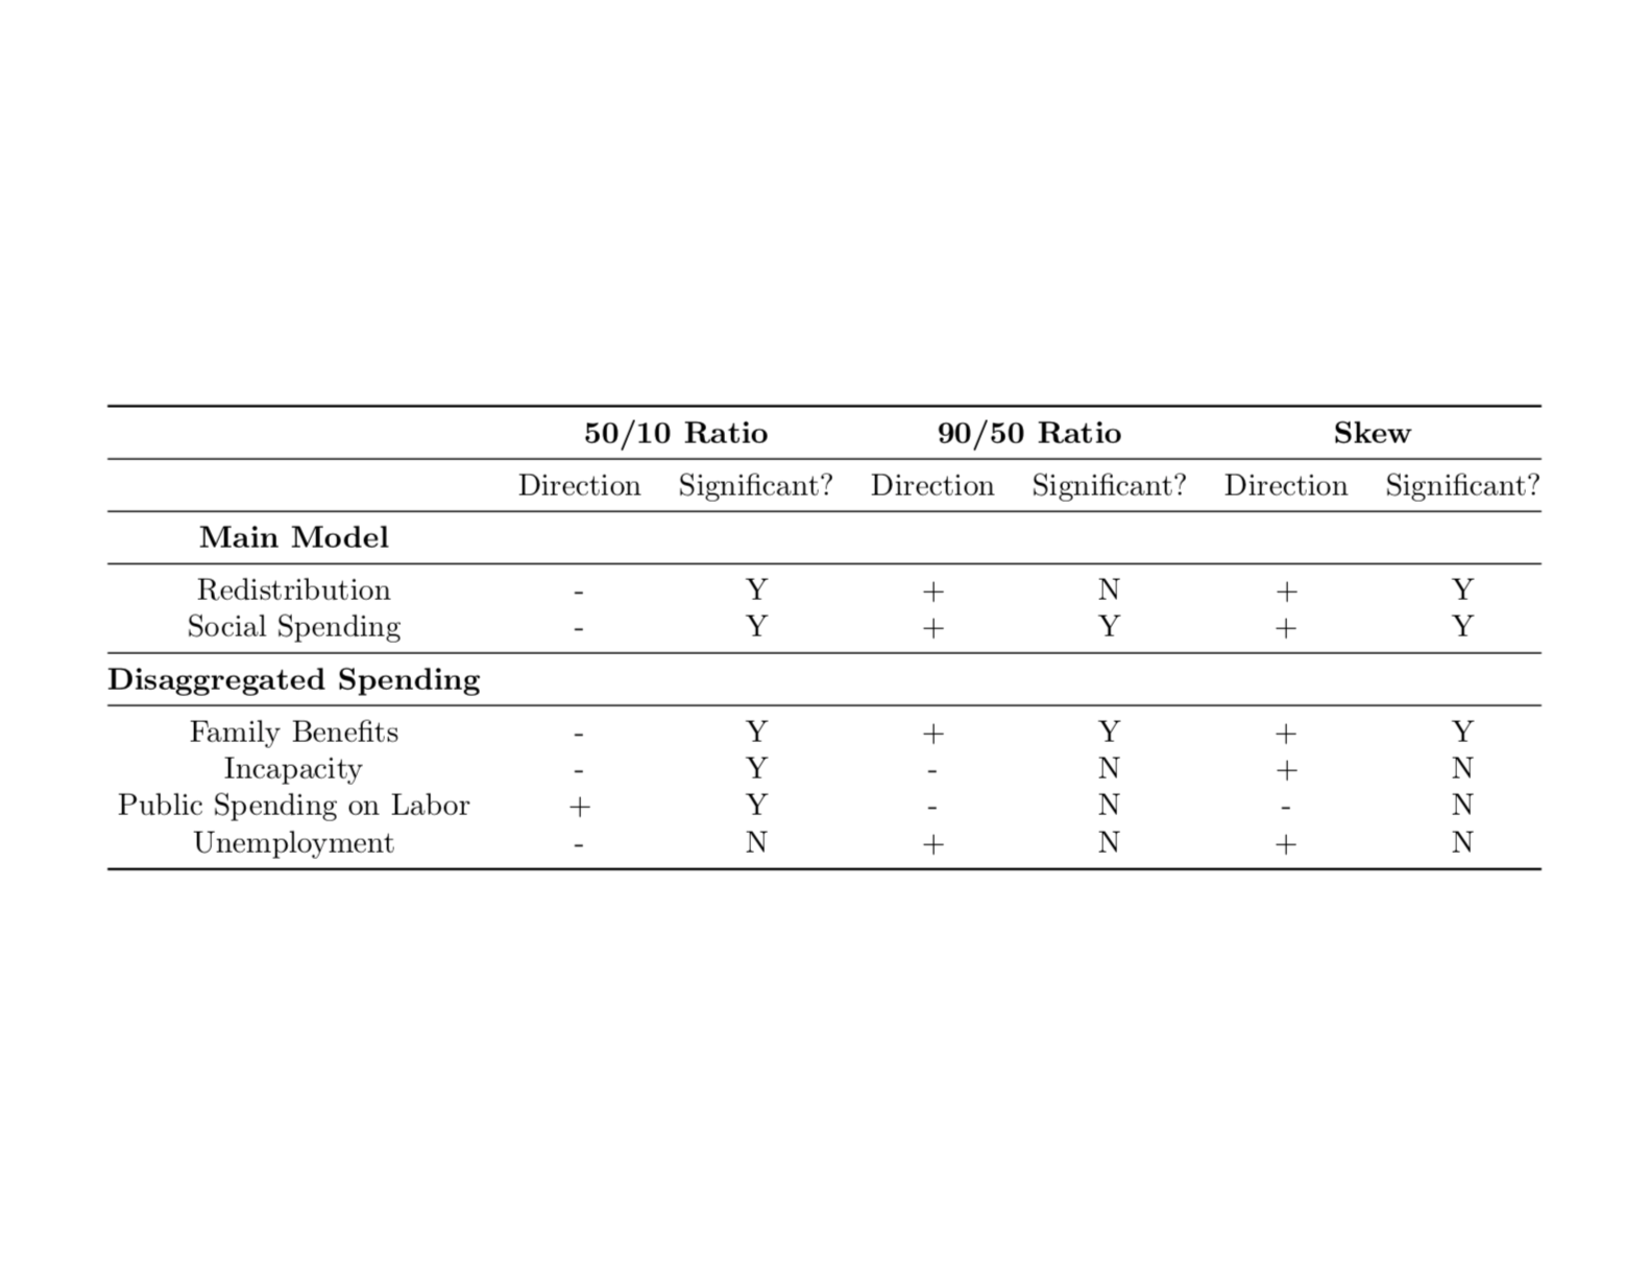
\includegraphics[scale=0.4]{robustnesscheck1}
\end{center}
\end{frame}

\begin{frame}
\frametitle{Additional Robustness Results 1/2}
\begin{center}
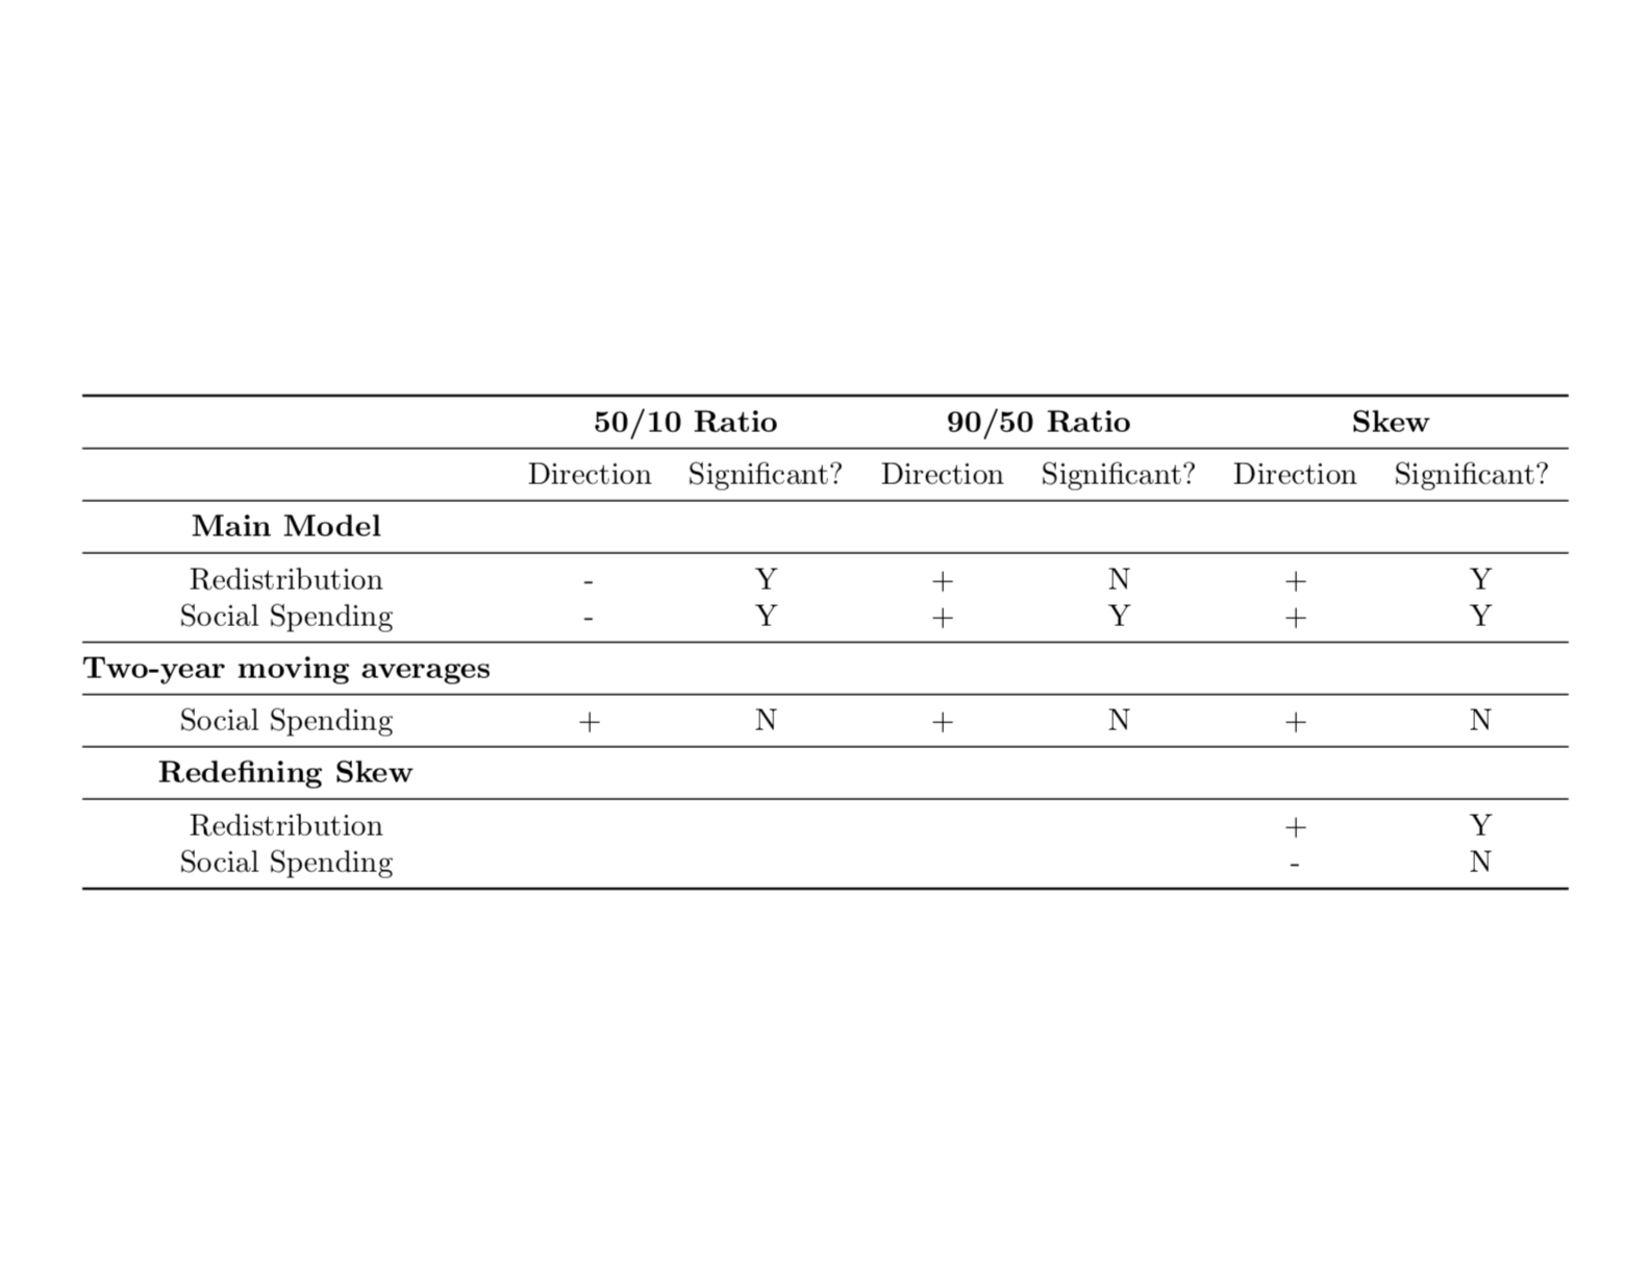
\includegraphics[scale=0.4]{robustnesscheck2}
\end{center}
\end{frame}

\begin{frame}
\frametitle{Additional Robustness Results 2/2}
\begin{center}
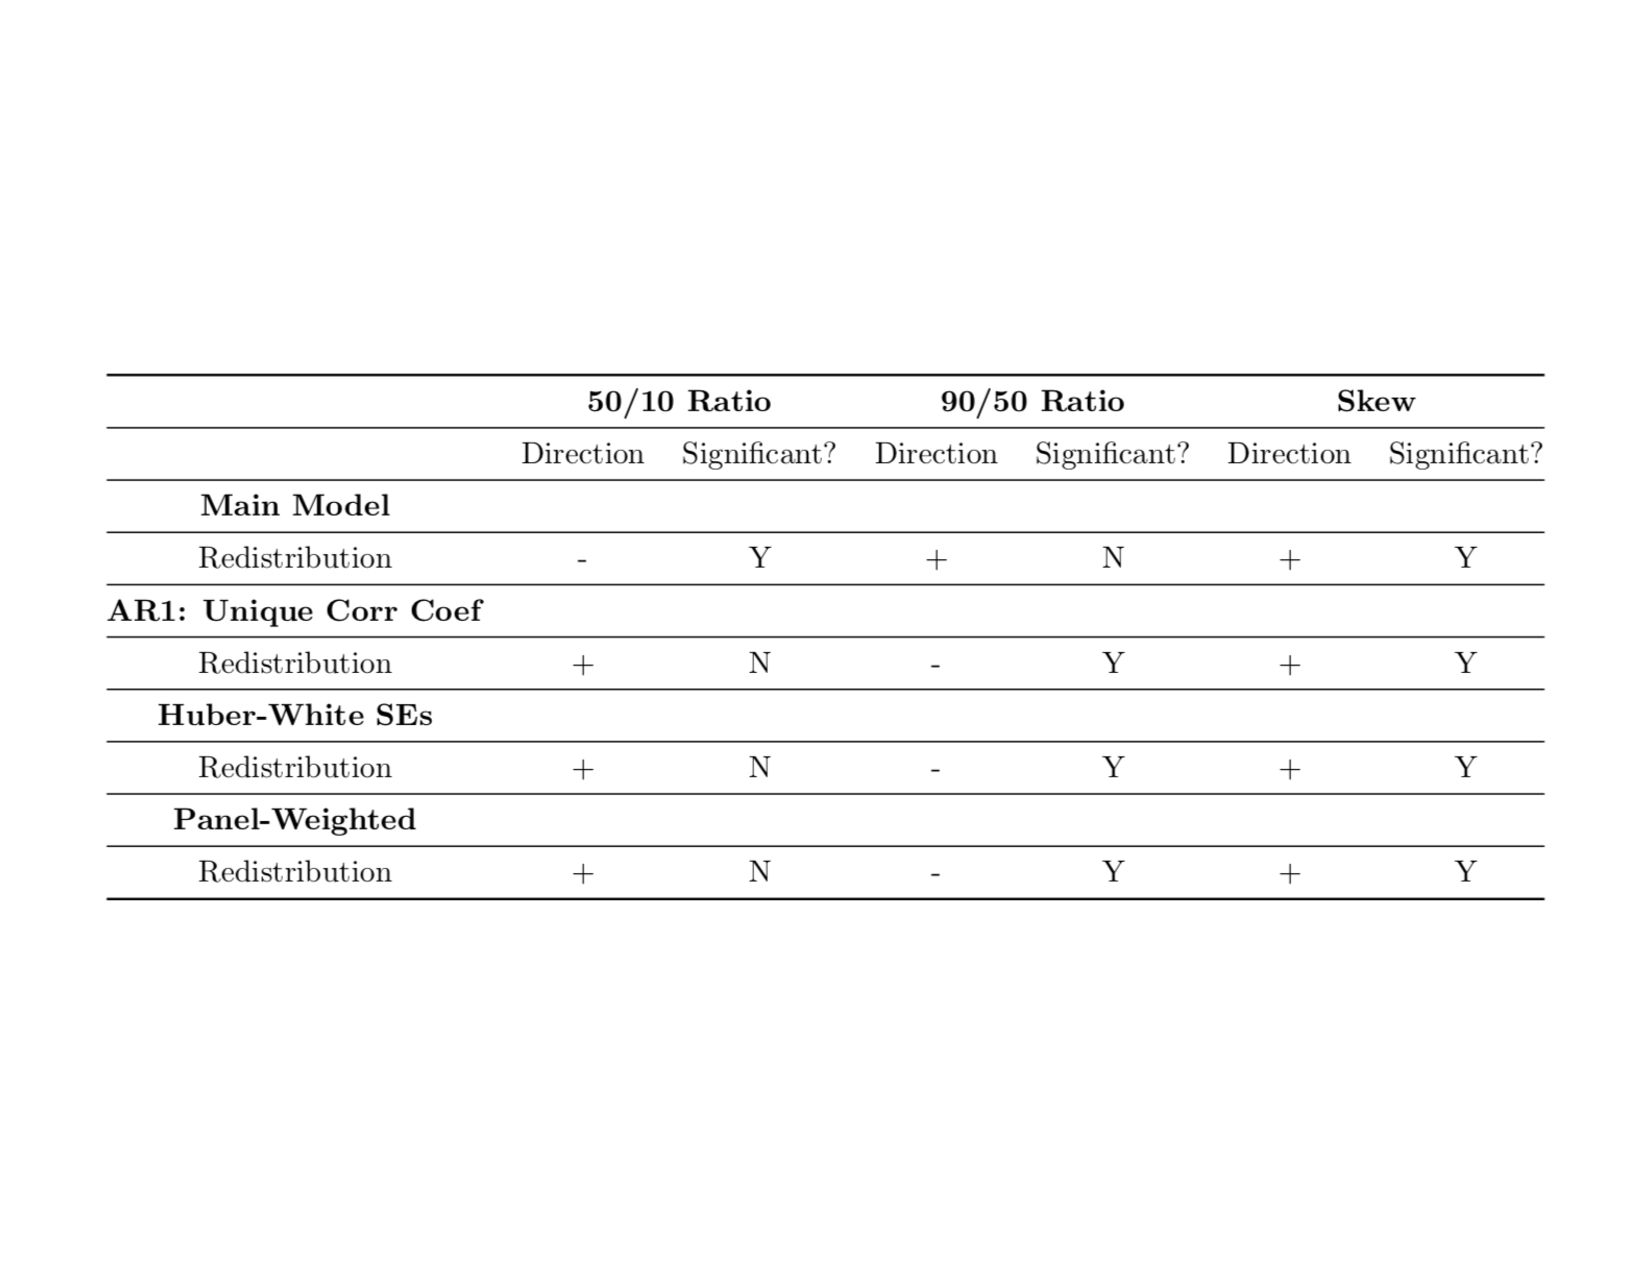
\includegraphics[scale=0.4]{robustnesscheck3}
\end{center}
\end{frame}

\begin{frame}
\subsection{Appendix}
appendix
\end{frame}

\begin{frame}
\frametitle{Empirical results}
$\longrightarrow$  What about preferences of middle-income voters?
\medskip
\begin{itemize}
\item[(i)] Correlation (R =.45) btw the \textbf{inequality} and \textbf{support for redistribution} of the middle-income voters  
\item[(ii)] Correlation (R =.43)  btw the \textbf{preference} of middle-income voters and \textbf{redistributive policies} pursued by government
\item[(iii)] Skewed \textbf{earnings inequality} promotes \textbf{left participation} in government ($R^{2}$ = .12)
\end{itemize}
\medskip
\begin{center}
= Preliminary result (see R and $R^{2}$ level)\\
\end{center}
\end{frame}
\begin{frame}
\frametitle{Conclusion}
\begin{itemize}
\item[1.] The structure of \textbf{inequality} is statistically and significantly associated with more \textbf{redistribution and social spending}
\medskip
\medskip
\medskip
\item[2.] \textbf{Middle-income voters} are incline to allay with low-income voters and support redistributive policies when the distance between the middle and the poor is small (relative to the distance between the middle and the upper)
\medskip
\medskip
\medskip
\item[3.] \textbf{Left-leaning government} are more likely to redistribute income than right-leaning government and that governments are more likely to be left-leaning when the structure of inequality is skewed
\end{itemize}
\end{frame}

\begin{frame}
\frametitle{Critiques}
\begin{itemize}
\item[$\longrightarrow$]\textbf{Data limitation}: fewer than 10 observation for earning inequalities for 6 over 15 countries
\item[$\longrightarrow$] \textbf{Geography}: If median = middle voters, how these results are consistent in developing countries in which the middle class is typically small (Houle, 2015)?
\item[$\longrightarrow$] \textbf{Ethnicity}: Class expressed as a racial group in developed countries? Racial minorities are highly over-represented among the poorest (Alesina and Glaeser, 2004)
\item[$\longrightarrow$] How \textbf{political instability} - that influence income inequalities (Perotti, 1995: Alesina \& Perotti, 1994)- can affect the results? 
\end{itemize}
\end{frame}


\begin{frame}
\frametitle{Design declaration}\
\begin{itemize}
\item[a)] \textit{declare population} = Describes dimensions and distributions over the variables in the population  $\longrightarrow$ The study concerns\textbf{ country year units} (858 observations).
\item[b)] \textit{declare potential outcomes} = Takes population or sample and adds potential outcomes produced by interventions $\longrightarrow$ Does more \textbf{inequality lead to more redistribution}?  
\item[c)] \textit{declare sampling} = (takes a population and selects a sample)  $\longrightarrow$ \textbf{N = 858}
\item[d)] \textit{declare assignment} = (takes a population or sample and adds treatment assignments)  $\longrightarrow$ \textbf{XXX}
\item[e)]\textit{declare estimand} = (takes potential outcomes and calculates a quantity of interest) $\longrightarrow$ \textbf{OLS with robust standard errors}
\item[f)]\textit{declare estimator} = takes data produced by sampling and assignment and returns estimates) $\longrightarrow$ \textbf{average slope of effects?}
\end{itemize}
\end{frame}
\begin{frame}
\frametitle{References}
\footnotesize{
\begin{thebibliography}{99}
\bibitem[Lupu and Pontusson, 2011]{p1} Lupu and Pontusson (2011)
\newblock The structure of Inequalities and the Politics of Redistribution
\newblock \emph{American Political Science Review} 105(2), 316 -- 335.

\end{thebibliography}
}
\end{frame}

\end{document}
